\documentclass[border=12pt]{standalone}
\def\pgfsysdriver{pgfsys-dvisvgm.def}
\usepackage[dvisvgm]{xcolor}
\usepackage{xeCJK}
\setCJKmainfont{HaranoAjiGothic-Regular.otf}[BoldFont=HaranoAjiGothic-Bold.otf]
\setCJKsansfont{HaranoAjiGothic-Regular.otf}[BoldFont=HaranoAjiGothic-Bold.otf]
\usepackage{amsmath,amssymb,tikz,lmodern}
\usetikzlibrary{arrows.meta,positioning,calc,fit,backgrounds}
\renewcommand{\familydefault}{\sfdefault}
\definecolor{ink}{HTML}{25322F}
\definecolor{green}{HTML}{246657}
\definecolor{tint}{HTML}{EEF4F0}
\definecolor{soft}{HTML}{C6D2CC}
\definecolor{muted}{HTML}{52615B}
\newif\ifJapanese
\newcommand{\Tx}[2]{\ifJapanese #1\else #2\fi}
\newcommand{\Eff}{\overline{\operatorname{Eff}}}
\newcommand{\heading}[3]{{\color{green}\bfseries #1\quad\Tx{#2}{#3}}\\[5pt]}
% A white rectangle makes the complete citation label clickable, including spaces.
\newcommand{\refurl}[2]{\special{dvisvgm:raw <a xlink:href="#1" target="_blank" rel="noopener noreferrer">}{\setlength{\fboxsep}{0pt}\colorbox{white}{\color{green}\underline{\strut #2}}}\special{dvisvgm:raw </a>}}
\newcommand{\refedge}[3]{\refurl{\csname source#1\endcsname\string##page=#2}{#3}}
\newcommand{\SF}[2]{\refedge{sf}{#1}{#2}}
% GitHub's file preview does not support PDF page fragments.
\newcommand{\LA}[2]{\refurl{\sourcela}{#2}}
\newcommand{\Sch}[2]{\refedge{sch}{#1}{#2}}
\newcommand{\PS}[2]{\refedge{ps}{#1}{#2}}
\tikzset{
 card/.style={draw=soft,fill=white,rounded corners=2pt,align=left,text=ink,font=\fontsize{10.5}{14}\selectfont,inner xsep=12pt,inner ysep=10pt,text width=14.4cm},
 half/.style={card,text width=6.45cm,minimum height=2.05cm},
 result/.style={card,draw=green,fill=tint,line width=.9pt},
 reason/.style={align=left,text=muted,font=\fontsize{9}{12}\selectfont,inner sep=0pt,text width=12.7cm},
 branchreason/.style={reason,text width=5.95cm},
 edge/.style={-{Stealth[length=2.4mm]},draw=green,line width=1pt},
 wire/.style={draw=green,line width=1pt},
}
% Keep the arrow in a dedicated left gutter; explanations never cover it.
\newcommand{\flow}[3]{
 \coordinate (#2-from) at ($(#1.south)+(-6.9,0)$);
 \coordinate (#2-to) at ($(#2.north)+(-6.9,0)$);
 \draw[edge] (#2-from)--(#2-to);
 \node[reason,anchor=west] (#2-reason) at ($(#2-from)!.5!(#2-to)+(.55,0)$) {#3};
}

\newcommand{\Hash}[2]{\refurl{\sourcehash}{#2}}
\newcommand{\FGring}[2]{\refedge{rings}{#1}{#2}}
\newcommand{\FGglue}[2]{\refedge{glue}{#1}{#2}}
\newcommand{\OI}[2]{\refurl{\sourceoi}{#2}}

\Japanesetrue
\newcommand{\sourcela}{https://github.com/openai/math/blob/adc7f1241b42e322a6451854ab7e4b4c146bf78a/preprints/Log-abundance-in-characteristic-zero-September-24-2026/paper.pdf}
\newcommand{\sourcehash}{https://arxiv.org/html/1609.00121v4}
\newcommand{\sourceglue}{https://www.math.kyoto-u.ac.jp/~fujino/fg-comp-final.pdf}
\newcommand{\sourcerings}{https://www.math.kyoto-u.ac.jp/~fujino/log-ring-aspm.pdf}
\newcommand{\sourceoi}{https://github.com/openai/math/blob/adc7f1241b42e322a6451854ab7e4b4c146bf78a/preprints/Orbifold-and-logarithmic-Iitaka-subadditivity-September-26-2026/paper.pdf}
\newcommand{\sourcehps}{https://people.math.harvard.edu/~mpopa/papers/HPS.pdf}
\newcommand{\sourcegmm}{https://github.com/openai/math/blob/adc7f1241b42e322a6451854ab7e4b4c146bf78a/preprints/Minimal-models-and-Mori-fibre-spaces-for-generalized-log-canonical-Q-pairs-September-24-2026/paper.pdf}
\begin{document}
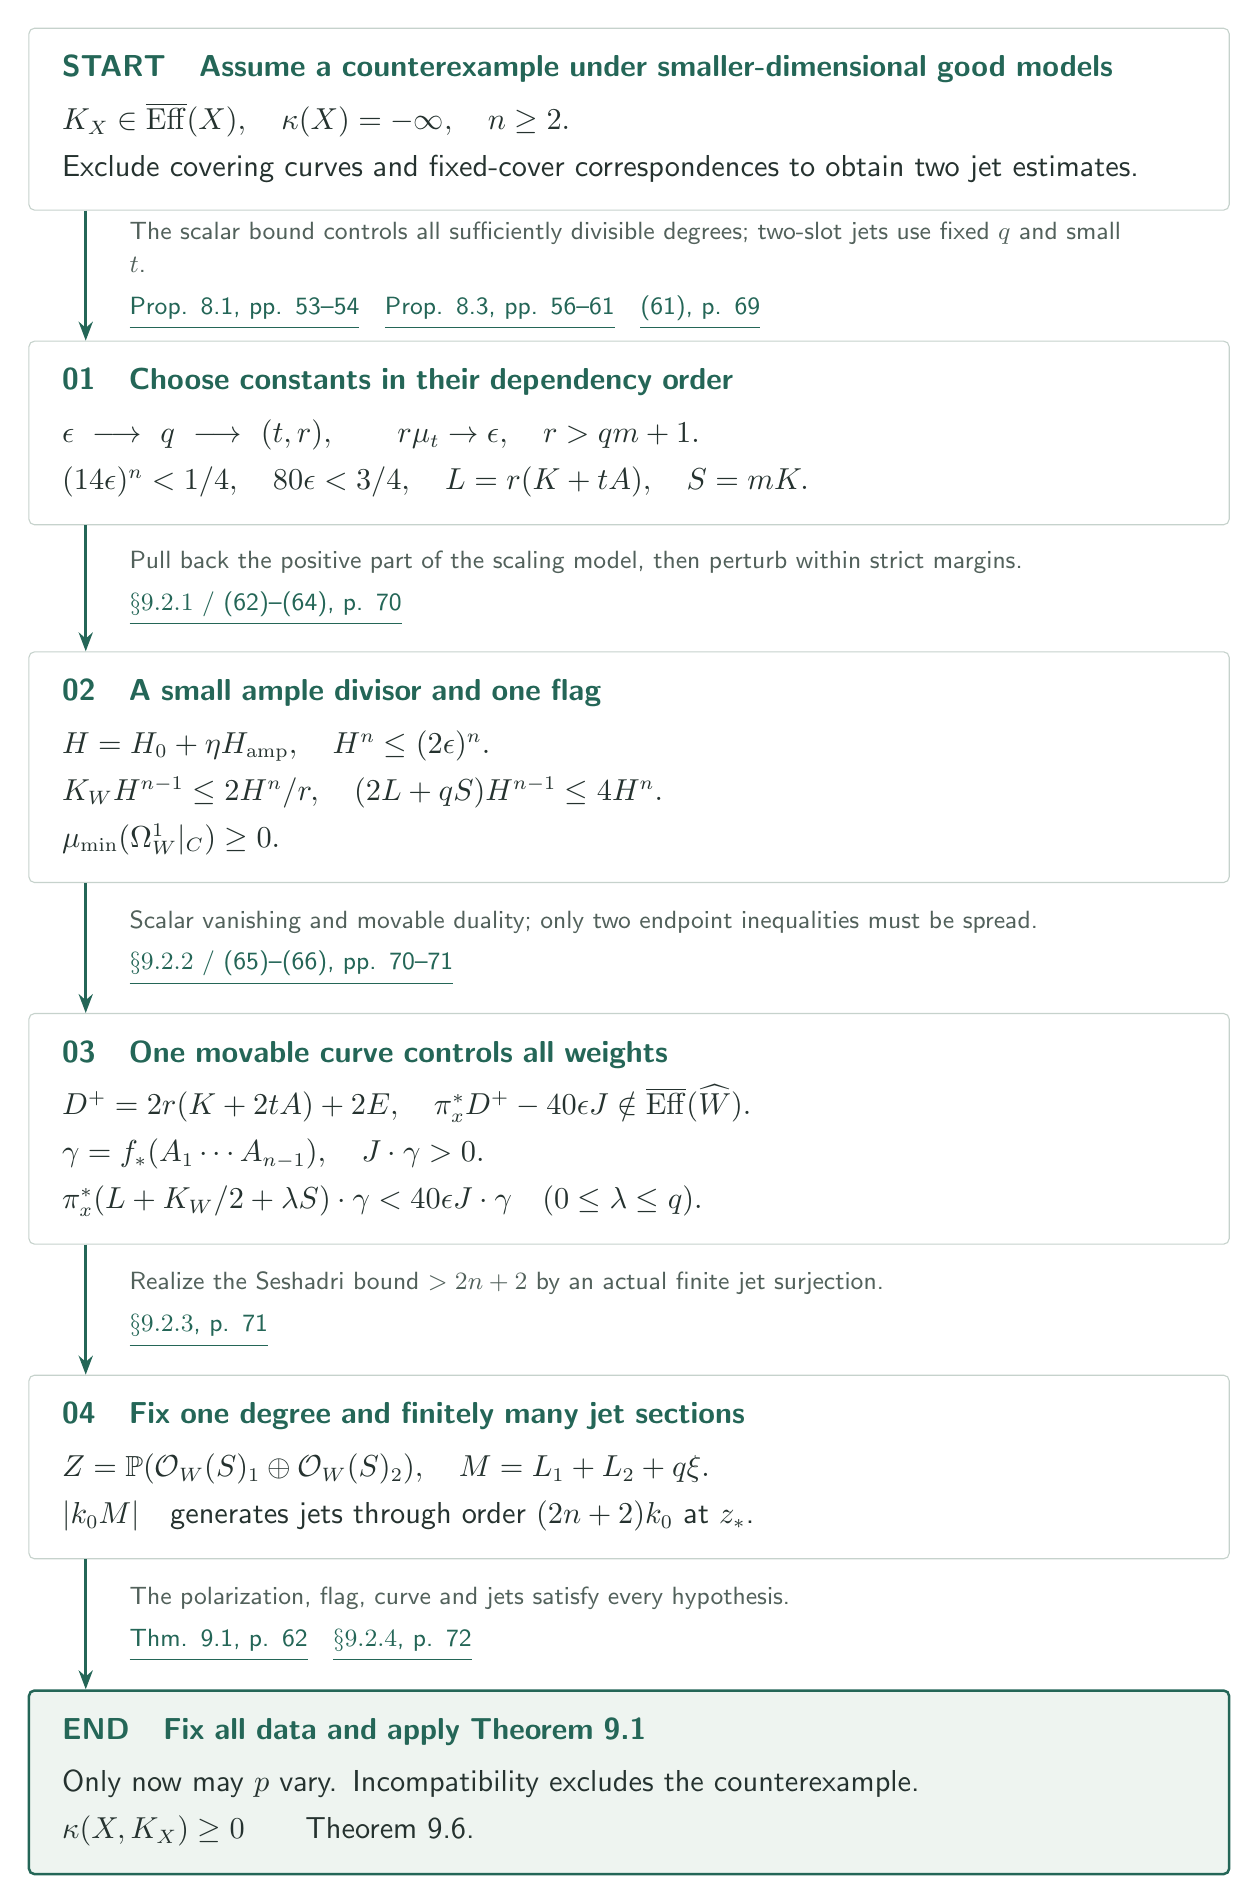
\begin{tikzpicture}
\node[card] (start) {\heading{START}{低次元の良いモデルの下で反例を仮定}{Assume a counterexample under smaller-dimensional good models}
$K_X\in\Eff(X),\quad\kappa(X)=-\infty,\quad n\geq2.$\\[3pt]
\Tx{被覆曲線・固定被覆の対応を排除し、二つのジェット評価を得る。}{Exclude covering curves and fixed-cover correspondences to obtain two jet estimates.}};
\node[card,below=1.65cm of start] (choice) {\heading{01}{定数を依存順に選ぶ}{Choose constants in their dependency order}
$\epsilon\ \longrightarrow\ q\ \longrightarrow\ (t,r),\qquad r\mu_t\to\epsilon,\quad r>qm+1.$\\[3pt]
$(14\epsilon)^n<1/4,\quad80\epsilon<3/4,\quad L=r(K+tA),\quad S=mK.$};
\flow{start}{choice}{\Tx{スカラー上界は十分可除な全次数、二因子評価は $q$ を固定して小さい $t$。}{The scalar bound controls all sufficiently divisible degrees; two-slot jets use fixed $q$ and small $t$.}\\[3pt]\LA{53}{Prop. 8.1, pp. 53--54}\quad\LA{56}{Prop. 8.3, pp. 56--61}\quad\LA{69}{(61), p. 69}}
\node[card,below=1.6cm of choice] (flag) {\heading{02}{小さい豊富因子と一つの旗}{A small ample divisor and one flag}
$H=H_0+\eta H_{\rm amp},\quad H^n\leq(2\epsilon)^n.$\\[3pt]
$K_WH^{n-1}\leq2H^n/r,\quad(2L+qS)H^{n-1}\leq4H^n.$\\[3pt]
$\mu_{\min}(\Omega_W^1|_C)\geq0.$};
\flow{choice}{flag}{\Tx{scaling model の正部分を引き戻し、厳密な余裕の範囲で豊富にする。}{Pull back the positive part of the scaling model, then perturb within strict margins.}\\[3pt]\LA{70}{$\S9.2.1$ / (62)--(64), p. 70}}
\node[card,below=1.65cm of flag] (curve) {\heading{03}{全重みを評価する一つの可動曲線}{One movable curve controls all weights}
$D^+=2r(K+2tA)+2E,\quad\pi_x^*D^+-40\epsilon J\notin\Eff(\widehat W).$\\[3pt]
$\gamma=f_*(A_1\cdots A_{n-1}),\quad J\cdot\gamma>0.$\\[3pt]
$\pi_x^*(L+K_W/2+\lambda S)\cdot\gamma<40\epsilon J\cdot\gamma\quad(0\leq\lambda\leq q).$};
\flow{flag}{curve}{\Tx{スカラー消滅上界と可動曲線双対性。還元に必要な条件は端点2個。}{Scalar vanishing and movable duality; only two endpoint inequalities must be spread.}\\[3pt]\LA{70}{$\S9.2.2$ / (65)--(66), pp. 70--71}}
\node[card,below=1.65cm of curve] (jets) {\heading{04}{一つの次数・有限個のジェット切断を固定}{Fix one degree and finitely many jet sections}
$Z=\mathbb P(\mathcal O_W(S)_1\oplus\mathcal O_W(S)_2),\quad M=L_1+L_2+q\xi.$\\[3pt]
$|k_0M|$\quad\Tx{が $z_*$ で次数 $(2n+2)k_0$ まで生成。}{generates jets through order $(2n+2)k_0$ at $z_*$.}};
\flow{curve}{jets}{\Tx{Seshadri 定数 $>2n+2$ を実際の有限ジェット全射にする。}{Realize the Seshadri bound $>2n+2$ by an actual finite jet surjection.}\\[3pt]\LA{71}{$\S9.2.3$, p. 71}}
\node[result,below=1.65cm of jets] (end) {\heading{END}{全データを固定して Theorem 9.1 に渡す}{Fix all data and apply Theorem 9.1}
\Tx{標数 $p$ を動かすのはこの後。両立不可能性が反例を排除する。}{Only now may $p$ vary. Incompatibility excludes the counterexample.}\\[3pt]
$\kappa(X,K_X)\geq0\qquad\text{Theorem 9.6.}$};
\flow{jets}{end}{\Tx{偏極・旗・可動曲線・ジェットが定理の全仮定を満たす。}{The polarization, flag, curve and jets satisfy every hypothesis.}\\[3pt]\LA{62}{Thm. 9.1, p. 62}\quad\LA{72}{$\S9.2.4$, p. 72}}
\end{tikzpicture}

\end{document}
